% HiddenPower — итерация 10, V01.
% Глава: «Практические проекты».
% Основная сквозная задача: консольная балка.
% Контрольная задача: MBB-балка.
% Архитектура главы:
% FEM + SIMP -> neural operator -> conditional diffusion + FEM + SIMP refinement.

\chapter{Практические проекты}
\label{chap:practical-projects}

Предыдущие главы уже дали математические и вычислительные инструменты, необходимые для практической работы: физические модели, численные решатели, дифференцирование и обучаемые методы. Здесь новая теория не вводится. Цель главы --- собрать эти средства в законченные вычислительные проекты и для каждого пройти путь от инженерной постановки до независимой проверки результата.

Во всех проектах рассматривается один класс задач линейной упругости. Основной сквозной пример --- прямоугольная консоль с закреплением части границы и внешней силой на свободной стороне. Внутри проектной области требуется распределить заданный объём материала. На этой задаче можно последовательно проверить граничные условия, сборку матрицы жёсткости, решение равновесия, податливость, чувствительность по плотности и выполнение ограничения объёма.

Второй механический сценарий --- MBB-балка, стандартная контрольная задача топологической оптимизации. Она не заменяет основной пример и не разворачивается во второй независимый проект. Её роль --- проверить переносимость реализации: тот же FEM- и SIMP-код должен работать после изменения геометрии закреплений и нагрузки, а последующие обучаемые модели не должны оцениваться только на конфигурации, максимально похожей на единственную исходную консоль.

Сквозная логика главы имеет вид
\begin{equation}
\label{eq:practical-projects-pipeline}
 \begin{gathered}
  \text{точная физика и оптимизация}
  \longrightarrow
  \text{обучаемый физический суррогат}
  \\
  \longrightarrow
  \text{генерация кандидатов с физической проверкой}.
 \end{gathered}
\end{equation}
Первый проект создаёт проверенный физический baseline и источник данных. Второй использует эти данные для приближения физического отображения. Третий решает уже не задачу предсказания, а задачу генерации конструкции и возвращает точный FEM-расчёт в контур как окончательный критерий качества. Поэтому каждый следующий проект зависит от предыдущего вычислительно, а не только тематически.

\section{Сквозной экспериментальный протокол}
\label{sec:practical-experimental-protocol}

Пусть $D\subset\R^2$ --- прямоугольная проектная область, $\mathcal T_h$ --- её конечно-элементная сетка, а
\begin{equation}
 \rho_h=(\rho_1,\ldots,\rho_N)
\end{equation}
--- вектор относительных плотностей элементов. Условие задачи обозначается через $c$ и содержит то, что алгоритм проектирования не выбирает: закрепления, внешнюю нагрузку и допустимую долю материала. Для фиксированных $(\rho_h,c)$ точный дискретный расчёт определяется системой
\begin{equation}
\label{eq:practical-fem-state}
 K_{ff}(\rho_h;c)U_f=F_f(c),
\end{equation}
а основной критерий качества --- податливость
\begin{equation}
\label{eq:practical-compliance}
 J_h(\rho_h;c)
 =
 F_h(c)^{\trans}U_h.
\end{equation}
Эти формулы уже были разобраны в главах о механике и генеративном проектировании; здесь они становятся программным контрактом. Любая конструкция, независимо от того, получена ли она SIMP-оптимизацией, нейронной сетью или диффузионной моделью, перед окончательным сравнением должна быть приведена к одному представлению $\rho_h$ и проверена одним физическим решателем.

\subsection{Основная и контрольная механические задачи}

Для консоли сохраняется одна и та же прямоугольная проектная область, а семейство условий $c$ строится изменением нагрузки и допустимой доли материала. Точные размеры сетки, величина силы, диапазон её положения и набор значений объёмной доли фиксируются в проекте~1 перед первой реализацией. После этого они не меняются молча между FEM, обучением суррогата и генеративным экспериментом.

MBB-задача используется как контрольная конфигурация с другим набором закреплений и нагрузки. Основной код не должен содержать специальных ветвей вида ``если консоль, то собрать систему иначе''. Различие между задачами должно проходить через данные $c$: список закреплённых степеней свободы, вектор внешних сил и параметры ограничения объёма. Такой интерфейс одновременно делает физический решатель переиспользуемым и подготавливает условие для последующих ML-моделей.

\subsection{Численная проверка физического расчёта}

После решения~\eqref{eq:practical-fem-state} вычисляется относительная невязка равновесия
\begin{equation}
\label{eq:practical-equilibrium-residual}
 r_{\mathrm{eq}}
 =
 \frac{
 \norm{K_{ff}U_f-F_f}_2
 }{
 \max(\norm{F_f}_2,\varepsilon)
 }.
\end{equation}
Здесь индекс $f$ относится к свободным степеням свободы. Полная разность $K_hU_h-F_h$ вообще не обязана быть нулевой: на закреплённых степенях свободы она содержит реакции опор. Малое $\varepsilon>0$ защищает только от деления на нуль в вырожденном тесте. Поэтому невязка~\eqref{eq:practical-equilibrium-residual} проверяет решение линейной системы, а реакции используются для отдельной проверки глобального баланса сил.

\begin{equation}
\label{eq:practical-volume-error}
 e_{\mathrm{vol}}
 =
 \left|
 \frac{1}{N}\sum_{e=1}^{N}\rho_e
 -
 f_{\mathrm{vol}}
 \right|,
\end{equation}
где $f_{\mathrm{vol}}$ --- заданная доля материала. В проекте~1 эта величина проверяет оптимизатор, в проекте~3 --- допустимость результата генератора после приведения к физическому представлению.

\subsection{Единица сравнения для ML-методов}

Обучаемая модель не считается проверенной по значению training loss. Для суррогата физического решения главным объектом сравнения остаётся точный FEM-результат. Если модель предсказывает поле перемещений $\widehat U_h$, используется относительная ошибка
\begin{equation}
\label{eq:practical-field-error}
 e_U
 =
 \frac{\norm{\widehat U_h-U_h}_2}
 {\max(\norm{U_h}_2,\varepsilon)}.
\end{equation}
Если по предсказанному состоянию вычисляется податливость $\widehat J_h$, дополнительно фиксируется относительная ошибка
\begin{equation}
\label{eq:practical-compliance-error}
 e_J
 =
 \frac{|\widehat J_h-J_h|}
 {\max(|J_h|,\varepsilon)}.
\end{equation}
Эти две ошибки отвечают на разные вопросы: малая ошибка критерия не гарантирует правильного поля, а хорошее среднее восстановление поля не гарантирует достаточной точности именно проектного функционала.

Для генеративной модели итоговой единицей сравнения становится не расстояние между изображениями плотности, а физически проверенный кандидат. Пусть $\rho_h^{\mathrm{gen}}$ --- сгенерированная конструкция, а $\rho_h^{\mathrm{ref}}$ --- та же конструкция после короткого SIMP-уточнения. Тогда эффект уточнения измеряется, например, относительным изменением
\begin{equation}
\label{eq:practical-refinement-gain}
 g_J
 =
 \frac{
 J_h(\rho_h^{\mathrm{gen}};c)
 -
 J_h(\rho_h^{\mathrm{ref}};c)
 }{
 \max(J_h(\rho_h^{\mathrm{gen}};c),\varepsilon)
 }.
\end{equation}
Положительное $g_J$ означает, что короткое физическое уточнение уменьшило податливость. Само по себе это ещё не делает генератор полезным: дополнительно сравниваются допустимость, время получения кандидата и качество относительно классического baseline.

\subsection{Воспроизводимость}

Каждый запускаемый эксперимент должен определять условие $c$, дискретизацию, параметры алгоритма и источник случайности. Случайный seed фиксируется там, где он влияет на генерацию данных, инициализацию сети или sampling. Численные результаты, используемые в тексте, должны восстанавливаться из кода главы без ручного редактирования массивов или переноса чисел из стороннего интерфейса.

Сгенерированные датасеты, веса моделей и промежуточные изображения не являются исходным кодом проекта и не должны бесконтрольно попадать в Git. В репозитории сохраняются реализация, конфигурация запуска и небольшие итоговые таблицы или рисунки, необходимые для воспроизведения текста. Большие производные данные должны создаваться повторным запуском соответствующего этапа.

\section{Проект 1. FEM и классическая топологическая оптимизация}
\label{sec:practical-project-fem-simp}

Первый проект начинается не с оптимизации, а с отдельной проверки механического решателя. SIMP многократно вызывает FEM внутри итерационного цикла, поэтому ошибка сборки или граничных условий затем будет выглядеть как свойство оптимизатора. На шаге V02 проектные плотности ещё не изменяются: вся область считается сплошным материалом. Ограничение объёма $f_{\mathrm{vol}}=0.4$ уже хранится в условии задачи, но начнёт действовать после подключения SIMP.

\subsection{Дискретная модель консоли}
\label{subsec:practical-v02-cantilever}

Проектная область выбрана в безразмерном виде,
\begin{equation}
\label{eq:practical-v02-domain}
 D=[0,3]\times[0,1].
\end{equation}
Она разбивается на $96\times32$ одинаковых четырёхузловых элементов. Поэтому
\begin{equation}
 h_x=\frac{3}{96}=\frac{1}{32},
 \qquad
 h_y=\frac{1}{32},
\end{equation}
то есть элементы квадратные. Сетка содержит $3072$ элемента, $3201$ узел и $6402$ степени свободы: в каждом узле вычисляются горизонтальное и вертикальное перемещения.

Модель соответствует тонкой плоской конструкции в состоянии плоского напряжения. Используются
\begin{equation}
\label{eq:practical-v02-material}
 E_0=1,
 \qquad
 \nu=0.3,
 \qquad
 t=1.
\end{equation}
Безразмерный выбор $E_0=1$ фиксирует масштаб жёсткости. При сравнении топологий в одной постановке нас интересуют относительные изменения податливости. Для плоского напряжения матрица закона Гука имеет вид
\begin{equation}
\label{eq:practical-v02-plane-stress}
 C
 =
 \frac{E_0}{1-\nu^2}
 \begin{pmatrix}
  1 & \nu & 0\\
  \nu & 1 & 0\\
  0 & 0 & \dfrac{1-\nu}{2}
 \end{pmatrix}.
\end{equation}

На каждом Q4-элементе перемещение билинейно интерполируется по четырём узлам, а интеграл жёсткости вычисляется квадратурой Гаусса $2\times2$. Для элемента $e$
\begin{equation}
\label{eq:practical-v02-element-stiffness}
 K_e
 =
 \int_{D_e}
 B_e^{\trans} C B_e\, t\, dA,
\end{equation}
где $B_e$ переводит узловые перемещения элемента в компоненты малой деформации. В коде интеграл~\eqref{eq:practical-v02-element-stiffness} вычисляется в четырёх гауссовых точках. Поскольку сетка равномерная, геометрическая матрица одного элемента переиспользуется при глобальной сборке.

Для основной консоли на всей левой границе $x=0$ задаются
\begin{equation}
\label{eq:practical-v02-cantilever-bc}
 u_x=u_y=0.
\end{equation}
Единичная сила направлена вниз и приложена в середине правой границы:
\begin{equation}
\label{eq:practical-v02-cantilever-load}
 F_x=0,
 \qquad
 F_y=-1.
\end{equation}
Положение и направление силы не зашиты в сборку матрицы. Функция условия принимает относительную высоту точки нагрузки и её угол, поэтому позднее тот же решатель сможет генерировать данные для различных $c$ без изменения FEM-ядра.

\subsection{Как учитываются закрепления}
\label{subsec:practical-v02-dirichlet}

После глобальной сборки степени свободы разделяются на свободные $f$ и закреплённые $c$. Для нулевых заданных перемещений $U_c=0$ полная система записывается как
\begin{equation}
 \begin{pmatrix}
  K_{ff} & K_{fc}\\
  K_{cf} & K_{cc}
 \end{pmatrix}
 \begin{pmatrix}
  U_f\\
  0
 \end{pmatrix}
 =
 \begin{pmatrix}
  F_f\\
  F_c+R_c
 \end{pmatrix},
\end{equation}
где $R_c$ --- реакции закреплений. Реально решается только система~\eqref{eq:practical-fem-state}. После нахождения $U_f$ полный вектор $U_h$ восстанавливается добавлением нулей на закреплённых степенях свободы, а реакции вычисляются из $K_hU_h-F_h$.

Проверять норму полного вектора $K_hU_h-F_h$ как невязку нельзя: на опорах она должна содержать ненулевую реакцию. В тестах используется свободная невязка~\eqref{eq:practical-equilibrium-residual}, а сумма внешних сил и реакций проверяется отдельно.

\subsection{Контрольная задача half-MBB}
\label{subsec:practical-v02-mbb}

Вторая постановка использует ту же область, сетку, материал и функцию сборки. Меняется только условие $c$. На левой границе фиксируется горизонтальное перемещение,
\begin{equation}
 u_x(0,y)=0,
\end{equation}
в правом нижнем узле дополнительно задаётся $u_y=0$, а единичная вертикальная сила вниз прикладывается в левом верхнем узле. Это half-MBB-конфигурация: левая граница играет роль плоскости симметрии, а одиночное вертикальное закрепление удаляет оставшееся жёсткое движение.

Практический смысл этой проверки не в получении второй картинки. Если для half-MBB приходится менять формулу элемента или писать отдельную сборку, интерфейс выбран неверно. В текущей реализации различаются только массив закреплённых степеней свободы и вектор $F_h$.

\subsection{Численные проверки V02}
\label{subsec:practical-v02-checks}

Сначала проверяется один свободный Q4-элемент. Его матрица жёсткости симметрична и имеет три нулевых собственных значения с машинной точностью. Они соответствуют двум переносам и одному повороту элемента как жёсткого тела. Остальные собственные значения положительны. После наложения корректных закреплений на малой тестовой сетке минимальное собственное значение $K_{ff}$ становится положительным.

На основной сетке $96\times32$ глобальная матрица содержит 105928 ненулевых коэффициентов. Для сплошной консоли получено
\begin{equation}
\label{eq:practical-v02-cantilever-result}
 J_h=118.276781,
 \qquad
 r_{\mathrm{eq}}=1.98e-12.
\end{equation}
Энергетическая проверка
\begin{equation}
\label{eq:practical-v02-energy-check}
 F_h^{\trans}U_h
 =
 U_h^{\trans}K_hU_h
 =
 2\,\Pi_{\mathrm{strain}}
\end{equation}
выполняется с относительной ошибкой 1.12e-12, а относительная ошибка глобального баланса сил равна 1.51e-11.

Тот же код без изменения элемента и сборки даёт для half-MBB
\begin{equation}
\label{eq:practical-v02-mbb-result}
 J_h=127.572691,
 \qquad
 r_{\mathrm{eq}}=2.78e-12.
\end{equation}
Ошибка энергетического тождества составляет 1.93e-13, ошибка баланса сил --- 2.70e-11. Различие значений $J_h$ ожидаемо: изменены опоры и точка приложения силы, хотя физическое ядро осталось тем же.

Эти числа не являются результатом топологической оптимизации. Они фиксируют контрольное состояние сплошного тела, относительно которого можно обнаружить поломку FEM после подключения проектных плотностей.


\subsection{SIMP: от плотности к жёсткости}
\label{subsec:practical-v03-simp}

После проверки FEM проектной переменной становится вектор $x=(x_1,\ldots,x_N)$, где $0\leq x_e\leq1$. Сам $x_e$ не подставляется в матрицу жёсткости напрямую. Сначала применяется density filter,
\begin{equation}
\label{eq:practical-v03-density-filter}
 \rho_i
 =
 \frac{\sum_j H_{ij}x_j}{\sum_j H_{ij}},
 \qquad
 H_{ij}
 =
 \max\{0,r_{\min}-d_{ij}\},
\end{equation}
где $d_{ij}$ --- расстояние между центрами элементов в единицах шага сетки. В основном запуске $r_{\min}=1.5$. Поэтому $\rho$ является физической плотностью, по которой одновременно вычисляются жёсткость и фактический расход материала.

SIMP-интерполяция имеет вид
\begin{equation}
\label{eq:practical-v03-simp-law}
 E_e
 =
 E_{\min}
 +
 \rho_e^p(E_0-E_{\min}),
 \qquad
 p=3,
 \qquad
 \frac{E_{\min}}{E_0}=10^{-9}.
\end{equation}
Малая остаточная жёсткость $E_{\min}$ не изображает реальный материал. Она не даёт глобальной матрице стать вырожденной, когда часть элементов приближается к пустоте. При $E_0=1$ множитель матрицы элемента равен $10^{-9}+(1-10^{-9})\rho_e^3$.

Оптимизационная задача для фиксированного условия $c$ записывается как
\begin{equation}
\label{eq:practical-v03-problem}
 \min_{0\leq x_e\leq1}
 J_h(\rho(x);c),
 \qquad
 \frac{1}{N}\sum_{e=1}^{N}\rho_e
 \leq
 f_{\mathrm{vol}},
 \qquad
 f_{\mathrm{vol}}=0.4.
\end{equation}
Начальная точка однородна: $x_e=0.4$. Поэтому первый FEM-расчёт уже относится не к сплошному телу V02, а к равномерно ослабленному SIMP-материалу.

\subsection{Производная и её численная проверка}
\label{subsec:practical-v03-gradient}

Для физической плотности производная податливости по элементу равна
\begin{equation}
\label{eq:practical-v03-physical-gradient}
 \frac{\partial J_h}{\partial\rho_e}
 =
 -p(E_0-E_{\min})
 \rho_e^{p-1}
 U_e^{\trans}K_e^{(0)}U_e,
\end{equation}
где $K_e^{(0)}$ --- матрица элемента при $E_0=1$, а $U_e$ содержит восемь степеней свободы этого элемента. Минус возникает из производной решения системы равновесия: увеличение жёсткости уменьшает податливость.

Фильтр~\eqref{eq:practical-v03-density-filter} является линейной картой $\rho=Dx$. Поэтому градиент по реальной проектной переменной получается не эвристической фильтрацией, а обычным правилом цепочки,
\begin{equation}
\label{eq:practical-v03-chain-rule}
 \nabla_x J_h
 =
 D^{\trans}\nabla_\rho J_h.
\end{equation}
Точно так же через $D^{\trans}$ переносится производная ограничения объёма. Это важно для дальнейшего использования датасета: сохранённое поле $\rho$ имеет один и тот же физический смысл в оптимизаторе и в будущей обучаемой модели.

Перед большим запуском производная проверена на сетке $12\times4$. Для шести компонент аналитический градиент сравнивался с центральной разностью
\begin{equation}
\label{eq:practical-v03-finite-difference}
 \frac{\partial J}{\partial x_i}
 \approx
 \frac{J(x+\delta e_i)-J(x-\delta e_i)}{2\delta},
 \qquad
 \delta=10^{-6}.
\end{equation}
Максимальная относительная ошибка составила 7.99e-06. Это отдельная проверка именно связки FEM, SIMP и density filter: корректная невязка линейной системы сама по себе правильность производной не подтверждает.

\subsection{OC-обновление и критерий остановки}
\label{subsec:practical-v03-oc}

Проектные переменные обновляются методом optimality criteria. Для фиксированного множителя $\lambda>0$ используется
\begin{equation}
\label{eq:practical-v03-oc-update}
 \begin{aligned}
 x_e^{\mathrm{trial}}
 &=
 x_e
 \sqrt{
 -\frac{\partial J/\partial x_e}
 {\lambda\,\partial V/\partial x_e}
 },\\
 x_e^{\mathrm{new}}
 &=
 \operatorname{clip}_{[0,1]}
 \left(
 \operatorname{clip}_{[x_e-m,x_e+m]}
 \left[x_e^{\mathrm{trial}}\right]
 \right).
 \end{aligned}
\end{equation}
где $m=0.2$ --- максимально разрешённое изменение одной переменной за итерацию. Множитель $\lambda$ находится бисекцией так, чтобы средняя физическая плотность после фильтра была равна $0.4$ с численной точностью.

Итерации прекращаются, когда
\begin{equation}
 \max_e|x_e^{(k+1)}-x_e^{(k)}|<10^{-2},
\end{equation}
или после $250$ шагов. Этот критерий не утверждает, что найден глобальный минимум невыпуклой SIMP-задачи. Он только фиксирует воспроизводимое окончание выбранного локального алгоритма.

\subsection{Результат для консоли и half-MBB}
\label{subsec:practical-v03-results}

Для основной консоли начальная равномерная конструкция при $f_{\mathrm{vol}}=0.4$ имеет
\begin{equation}
 J_h^{(0)}=1848.074672.
\end{equation}
После 77 OC-итераций получено
\begin{equation}
\label{eq:practical-v03-cantilever-final}
 J_h=233.550039,
 \qquad
 \overline{\rho}=0.400000000,
 \qquad
 \max|\Delta x|=9.612e-03.
\end{equation}
Податливость уменьшилась на 87.4\% относительно равномерного распределения тех же $40\%$ материала. Относительная невязка конечного FEM-решения равна 1.78e-12.

Для контрольной half-MBB тот же код, те же $p$, $r_{\min}$ и OC-параметры дают после 222 итераций
\begin{equation}
\label{eq:practical-v03-mbb-final}
 J_h=260.048345,
 \qquad
 \overline{\rho}=0.400000000,
 \qquad
 \max|\Delta x|=9.674e-03.
\end{equation}
Начальная податливость здесь равна 1993.323267, а относительное уменьшение --- 87.0\%. Независимость оптимизационного ядра от типа опор сохраняется: меняется объект условия $c$, но не формулы FEM, фильтра, производной или OC.

\begin{figure}[ht]
 \centering
 \begin{minipage}{0.48\textwidth}
  \centering
  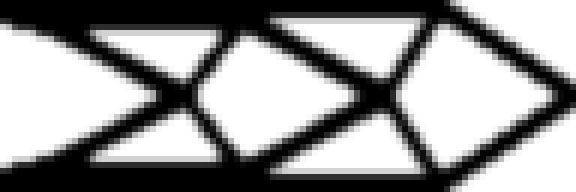
\includegraphics[width=\linewidth]{figures/ch10_v03_cantilever_density.png}
 \end{minipage}
 \hfill
 \begin{minipage}{0.48\textwidth}
  \centering
  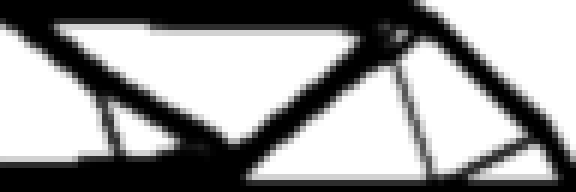
\includegraphics[width=\linewidth]{figures/ch10_v03_half_mbb_density.png}
 \end{minipage}
 \caption{Физическая плотность после SIMP-оптимизации: основная консоль слева и контрольная half-MBB справа. Чёрный цвет соответствует материалу, белый --- пустоте.}
 \label{fig:practical-v03-topologies}
\end{figure}

Рисунок~\ref{fig:practical-v03-topologies} нужен не вместо численной проверки, а вместе с ней. В файле результатов сохраняются объём, податливость, невязка, энергетическое тождество и история итераций. Поэтому визуально правдоподобная топология не может скрыть нарушение физического ограничения или ошибку решателя.

\subsection{Что показывает повторный расчёт на другой сетке}
\label{subsec:practical-v03-mesh-check}

Оптимизация выполнялась только на основной сетке $96\times32$. Чтобы отдельно оценить чувствительность физического расчёта к дискретизации, найденное поле $\rho$ консоли без новой оптимизации переносится на две сетки. Для $48\times16$ каждые четыре плотности усредняются, а для $192\times64$ каждая плотность копируется в четыре дочерних элемента. Средняя плотность при обеих операциях остаётся равной $0.4$.

Повторный FEM даёт
\begin{equation}
\label{eq:practical-v03-mesh-check}
 \begin{aligned}
  J_{48\times16} &= 254.061339,\\
  J_{96\times32} &= 233.550039,\\
  J_{192\times64} &= 239.409264.
 \end{aligned}
\end{equation}
На более тонкой сетке отклонение от основного расчёта составляет 2.51\%. Это не доказательство сеточной сходимости оптимальной топологии: на трёх сетках не решались три независимые задачи оптимизации. Проверка уже по смыслу --- она показывает, насколько меняется точная физическая оценка одного и того же найденного распределения при удвоении и уменьшении разрешения.

Итог проекта~1 теперь содержит полный проверяемый контур
\begin{equation}
 c
 \longrightarrow
 \rho^{(0)}
 \longrightarrow
 \mathrm{FEM}
 \longrightarrow
 \nabla J
 \longrightarrow
 \mathrm{filter+OC}
 \longrightarrow
 \rho^\star
 \longrightarrow
 \mathrm{FEM}.
\end{equation}
Именно этот solver в следующем проекте становится источником данных. Обучаемая модель будет сравниваться не с абстрактной ``правильной картинкой'', а с полями и функционалами, вычисленными здесь.


\section{Проект 2. Нейронный оператор как суррогат физического решателя}
\label{sec:practical-project-neural-operator}

Второй проект не пытается напрямую угадывать оптимальную конструкцию. Его задача уже: заменить многократно вызываемый физический расчёт приближённым отображением
\begin{equation}
\label{eq:practical-v04-operator-map}
 (\rho_h,c)\longmapsto U_h.
\end{equation}
Точный ответ по-прежнему задаётся FEM-системой~\eqref{eq:practical-fem-state}. Поэтому обучаемая модель будет сравниваться с собственным численным эталоном проекта~1, а не с визуальной похожестью полей.

\subsection{Почему в датасете нужны промежуточные конструкции}
\label{subsec:practical-v04-why-trajectories}

Если сохранить только финальные $\rho^\star$, выборка будет состоять в основном из хороших почти бинарных топологий. Однако суррогат нужен также для оценки промежуточных и сгенерированных кандидатов, где плотности могут быть серыми и податливость далека от оптимальной. Поэтому исходной единицей данных становится целая SIMP-траектория при фиксированном условии $c$.

Из каждой траектории выбираются шесть состояний с относительным прогрессом
\begin{equation}
\label{eq:practical-v04-snapshot-fractions}
 0,\qquad
 0.05,\qquad
 0.15,\qquad
 0.35,\qquad
 0.65,\qquad
 1.
\end{equation}
Первый снимок соответствует равномерной начальной плотности, последний --- состоянию после выполнения критерия $\max|\Delta x|<10^{-2}$. Остальные четыре точки покрывают различные стадии перераспределения материала. Верхний предел числа OC-итераций в генераторе равен $800$; это только защитный cap и он не меняет критерий остановки.

\subsection{Семейство условий}
\label{subsec:practical-v04-condition-grid}

Геометрия и закрепление консоли остаются теми же, что в проекте~1. Варьируются объёмная доля, высота точки приложения силы и её направление:
\begin{equation}
\label{eq:practical-v04-condition-grid}
 \begin{aligned}
 f_{\mathrm{vol}}
 &\in\{0.30,0.40,0.50\},\\
 y_F/H
 &\in\{0.25,0.50,0.75\},\\
 \theta_F
 &\in\{-105^\circ,-90^\circ,-75^\circ\}.
 \end{aligned}
\end{equation}
Полный декартов набор содержит $27$ условий. Угол в компактных метаданных кодируется парой $(\cos\theta_F,\sin\theta_F)$, поэтому
\begin{equation}
 q=
 \left(
 f_{\mathrm{vol}},
 \frac{y_F}{H},
 \cos\theta_F,
 \sin\theta_F
 \right).
\end{equation}

Все 27 траекторий достигли критерия остановки за $77$--$324$ OC-итерации; лимит $800$ ни разу не сработал. Максимальная относительная FEM-невязка сохранённых состояний равна $2.34e-12$.34e-12.

\subsection{Схема одного sample}
\label{subsec:practical-v04-sample-schema}

Физическая плотность естественно определена на элементах и имеет размер $32\times96$. Поле перемещений определено в узлах и имеет два компонента на сетке $33\times97$. Поэтому \texttt{rho\_element} хранит исходную физическую плотность, а \texttt{rho\_node} --- её локальное усреднение в узлы. Второе представление не заменяет первое; оно только переводит вход на ту же пространственную сетку, где задано целевое поле.

Сила хранится как два разреженных узловых канала, а два канала маски закреплений постоянны для всего семейства консолей. Цель имеет форму
\begin{equation}
 U_{\mathrm{data}}
 \in
 \mathbb{R}^{2\times33\times97}.
\end{equation}
Дополнительно сохраняются податливость, FEM-невязка, номер исходного условия, номер SIMP-итерации и относительный прогресс по траектории.

\subsection{Разделение без утечки траекторий}
\label{subsec:practical-v04-split}

Снимки одной SIMP-траектории близки, поэтому разделение выполняется по условиям $c$, а не по отдельным состояниям. Все шесть снимков одного условия целиком попадают в train, validation или test.

Из $27$ условий 18 используются для обучения, 4 для validation и 5 для test. При шести снимках на условие получаем
\begin{equation}
\label{eq:practical-v04-split-counts}
 N_{\mathrm{train}}=108,
 \qquad
 N_{\mathrm{val}}=24,
 \qquad
 N_{\mathrm{test}}=30,
\end{equation}
то есть всего 162 точных пар $(\rho_h,c,U_h)$. Автоматический аудит дополнительно проверяет, что один \texttt{condition\_id} никогда не встречается более чем в одном split.

\begin{figure}[ht]
 \centering
 
\includegraphics[width=\textwidth]{figures/ch10_v04_dataset_trajectory.png}
 \caption{Шесть сохранённых состояний одной SIMP-траектории для $f_{\mathrm{vol}}=0.4$, $y_F/H=0.5$, $\theta_F=-90^\circ$: от равномерной начальной плотности до терминальной конструкции.}
 \label{fig:practical-v04-trajectory}
\end{figure}

Рисунок~\ref{fig:practical-v04-trajectory} показывает, что будущая модель видит не только почти чёрно-белые оптимумы, но и промежуточные поля. Это соответствует её практической роли: быстро оценивать произвольный кандидат до дорогой окончательной физической проверки.

\subsection{Воспроизводимость датасета}
\label{subsec:practical-v04-reproducibility}

Полный бинарный датасет не сохраняется в Git. Он генерируется в каталоге \texttt{code/chapter10/data/} под именем \texttt{v04\_operator\_dataset.npz}. Его размер 5.34 MiB и SHA256
\begin{equation}
\label{eq:practical-v04-dataset-hash}
 \begin{gathered}
  \texttt{eeace8c3e22dd1ce0d3cb52bc05c0215}\\
  \texttt{88a948b02e2c74afc84545407f547385}.
 \end{gathered}
\end{equation}
В репозитории остаются генератор, список условий, seed разбиения, schema массивов и manifest с этим хешем. Поэтому данные можно воспроизвести и проверить, не превращая Git в хранилище бинарных обучающих массивов.

Следующий шаг использует именно этот train/validation/test split. Качество суррогата будет измеряться на условиях, исключённых из обучения, по относительной ошибке поля, ошибке податливости и физической невязке после подстановки предсказанного $U_h$ в точную FEM-систему.

\subsection{Fourier Neural Operator}
\label{subsec:practical-v05-fno}

После V04 вход и точный выход уже имеют согласованную пространственную структуру. Для суррогата используется компактный Fourier Neural Operator. В каждом скрытом слое локальное преобразование складывается со спектральным:
\begin{equation}
\label{eq:practical-v05-fno-layer}
 v_{k+1}
 =
 \sigma\!\left(
 W_k v_k
 +
 \mathcal{F}^{-1}
 \!\left[
 R_k\,\mathcal{F}v_k
 \right]
 \right).
\end{equation}
Здесь сохраняются только низкие Fourier-моды: $8$ по вертикальной и $16$ по горизонтальной координате. Ширина скрытого представления равна $24$, число Fourier-слоёв --- четыре. В итоге модель содержит 1184018 обучаемых действительных параметров.

Пространственный вход имеет девять каналов:
\begin{equation}
\label{eq:practical-v05-input}
 X_h=
 \left(
 \rho_h,\,
 F_x,\,
 F_y,\,
 x/L,\,
 y/H,\,
 f_{\mathrm{vol}},\,
 y_F/H,\,
 \cos\theta_F,\,
 \sin\theta_F
 \right).
\end{equation}
Последние четыре величины постоянны по пространству для одного sample. Выход содержит два канала $(\widehat u_x,\widehat u_y)$. Левое закрепление не изучается статистически: после последнего слоя выход умножается на маску свободных узлов, поэтому $\widehat u_x=\widehat u_y=0$ при $x=0$ выполняется точно.

\subsection{Обучение без доступа к test}
\label{subsec:practical-v05-training}

Статистики нормировки вычисляются только по $108$ train samples. Validation содержит $24$ состояния и выбирает checkpoint; $30$ test samples не участвуют ни в нормировке, ни в early stopping.

Оптимизация выполняется AdamW с начальным шагом $10^{-3}$ и weight decay $10^{-4}$. При отсутствии улучшения validation loss шаг уменьшается, а обучение останавливается досрочно. Лучший checkpoint получен на эпохе 160; всего выполнено 205 эпох. Минимальная validation-ошибка в нормированных переменных равна 0.0841. Полное обучение на CPU заняло 24.48 мин.

\subsection{Ошибка поля и инженерных величин}
\label{subsec:practical-v05-test}

Основная test-метрика вычисляется в физических перемещениях,
\begin{equation}
\label{eq:practical-v05-field-error}
 e_U
 =
 \frac{
 \norm{\widehat U_h-U_h}_2
 }{
 \norm{U_h}_2
 }.
\end{equation}
На $30$ test samples медиана $e_U$ равна 0.0368, а $90$-й процентиль --- 0.0919. Эти условия целиком отсутствовали в train split, поэтому результат нельзя объяснить запоминанием соседних состояний той же SIMP-траектории.

Для инженерной проверки одного совпадения формы поля недостаточно. По известному вектору нагрузки податливость FNO-предсказания вычисляется без нового FEM-решения:
\begin{equation}
 \widehat J_h
 =
 F_h^{\trans}\widehat U_h,
 \qquad
 e_J
 =
 \frac{
 |\widehat J_h-J_h|
 }{
 |J_h|
 }.
\end{equation}
Медианная относительная ошибка $e_J$ составляет 0.0733, $90$-й процентиль --- 0.2088.

Более строгая проверка подставляет предсказанное поле обратно в точную матрицу жёсткости:
\begin{equation}
\label{eq:practical-v05-physics-residual}
 r_{\mathrm{FNO}}
 =
 \frac{
 \norm{
 K_{ff}(\rho_h)\widehat U_f-F_f
 }_2
 }{
 \norm{F_f}_2
 }.
\end{equation}
Медиана этой невязки равна 6.45e+01, а $90$-й процентиль --- 8.64e+01. В отличие от ошибки поля, эта величина напрямую проверяет локальное равновесие. Поэтому малый $e_U$ сам по себе ещё не делает нейронный ответ заменой окончательной FEM-верификации.

\begin{figure}[ht]
 \centering
 
\includegraphics[width=\textwidth]{figures/ch10_v05_fno_test_example.png}
 \caption{Test-пример с ошибкой поля, близкой к медианной: слева точный модуль перемещения, в центре FNO-предсказание, справа модуль ошибки. Для первых двух панелей используется общий масштаб.}
 \label{fig:practical-v05-fno-example}
\end{figure}

\subsection{Стоимость и перенос разрешения}
\label{subsec:practical-v05-resolution}

На одном CPU и одном состоянии сетки $96\times32$ измеренный forward FNO занимает 32.553 мс, а полная сборка и решение FEM --- 171.536 мс. Их отношение в этом локальном измерении равно 5.27. Это не аппаратно-независимая оценка сложности, а практический wall-clock контроль конкретной реализации.

Fourier-слои не содержат параметров, привязанных к числу узлов, поэтому тот же checkpoint можно технически вызвать на другой регулярной сетке. Для exploratory-проверки одна терминальная test-конструкция перенесена с $96\times32$ на $192\times64$ элементов и повторно решена точным FEM. Без какого-либо fine-resolution обучения FNO дал
\begin{equation}
\label{eq:practical-v05-resolution-transfer}
 e_U^{192\times64}
 =
 0.3595,
 \qquad
 e_J^{192\times64}
 =
 0.2819.
\end{equation}
Физическая невязка на этой сетке равна 3.20e+02. Этот опыт проверяет возможность прямого вызова оператора на другом разрешении, но сам по себе не доказывает resolution invariance: для такого вывода нужен систематический эксперимент по нескольким условиям и сеткам.

Локальный checkpoint не хранится в Git. Его SHA256 разбит на две строки:
\begin{equation}
\label{eq:practical-v05-checkpoint-hash}
 \begin{gathered}
  \texttt{e3154c0cb697ee3abe8e9e83e7033ab9}\\
  \texttt{cf52f17495e98e431deeda17184e1608}.
 \end{gathered}
\end{equation}
В репозитории остаются архитектура, seed, история обучения и все test-метрики. Поэтому следующий шаг может отдельно разобрать зависимость ошибок от стадии SIMP, условия нагрузки и требуемой точности, не меняя уже обученный baseline.

\subsection{Где ошибается суррогат}
\label{subsec:practical-v06-error-structure}

После обучения архитектура и checkpoint больше не меняются. V06 повторно прогоняет те же $30$ test-состояний и разбивает ошибку по положению внутри SIMP-траектории. Это отделяет качество модели от процедуры выбора checkpoint.

\begin{table}[ht]
 \centering
 \small
 \begin{tabular}{c|c|c|c}
  прогресс & медиана $e_U$ & медиана $e_J$ & медиана $r_{\mathrm{FNO}}$\\
  \hline
  0.00 & 3.30\% & 3.85\% & 6.95e+01\\
  0.05 & 4.29\% & 6.96\% & 6.11e+01\\
  0.15 & 3.96\% & 8.08\% & 7.22e+01\\
  0.35 & 3.49\% & 7.98\% & 6.59e+01\\
  0.65 & 3.52\% & 7.70\% & 6.31e+01\\
  1.00 & 3.80\% & 7.69\% & 6.23e+01\\
 \end{tabular}
 \caption{Ошибка фиксированного FNO на шести стадиях test-траекторий. На каждой стадии присутствуют пять независимых условий.}
 \label{tab:practical-v06-stage-errors}
\end{table}

Минимальная медианная ошибка поля наблюдается на стадии 0, максимальная --- на стадии 1. Поэтому единственного числа $e_U$ недостаточно для описания качества: распределение конструкций меняется по мере SIMP-оптимизации, а вместе с ним меняется и трудность surrogate-задачи.

\subsection{Пять невидимых условий}
\label{subsec:practical-v06-condition-generalization}

Каждое test-условие содержит шесть состояний одной траектории. Полученные ошибки приведены отдельно:
\begin{table}[ht]
 \centering
 \small
 \begin{tabular}{c|c|c|c|c|c}
  $f_{\mathrm{vol}}$ & $y_F/H$ & $\theta_F$ & med $e_U$ & med $e_J$ & порядок $J$\\
  \hline
  0.30 & 0.50 & $-90^\circ$ & 2.79\% & 0.89\% & 100.0\%\\
  0.40 & 0.25 & $-90^\circ$ & 3.54\% & 1.66\% & 100.0\%\\
  0.40 & 0.25 & $-75^\circ$ & 9.60\% & 19.64\% & 73.3\%\\
  0.50 & 0.25 & $-90^\circ$ & 4.00\% & 7.69\% & 100.0\%\\
  0.50 & 0.75 & $-75^\circ$ & 2.98\% & 14.87\% & 100.0\%\\
 \end{tabular}
 \caption{Condition-level test: медианные ошибки и доля правильно упорядоченных пар кандидатов по податливости внутри одного условия.}
 \label{tab:practical-v06-condition-errors}
\end{table}

Эти пять строк нельзя интерпретировать как независимый эксперимент по влиянию $f_{\mathrm{vol}}$, положения силы или угла. Test subset специально отделён от train, но содержит только пять несбалансированных комбинаций параметров. Поэтому таблица показывает различия между конкретными невидимыми условиями, а не причинный эффект каждого параметра по отдельности.

\subsection{Почему малой ошибки поля недостаточно}
\label{subsec:practical-v06-physics-gap}

Для точного решения на свободных степенях свободы $K_{ff}U_f=F_f$. Если $\widehat U_f=U_f+\delta U_f$, то невязка surrogate равна
\begin{equation}
\label{eq:practical-v06-residual-error-link}
 K_{ff}\widehat U_f-F_f
 =
 K_{ff}\delta U_f.
\end{equation}
Поэтому относительная евклидова ошибка $\norm{\delta U}_2/\norm{U}_2$ и ошибка равновесия измеряют разные свойства. Матрица жёсткости усиливает те компоненты ошибки, которые дороги в энергетической норме. Именно поэтому медиана $e_U=0.0368$ может сосуществовать с медианной физической невязкой $64.5$.

На $30$ test samples корреляция между $e_U$ и $e_J$ равна 0.619, а между $e_U$ и $\log_{10}r_{\mathrm{FNO}}$ --- 0.466. Даже если эти величины меняются согласованно, ни одна из первых двух метрик не заменяет прямую проверку уравнения равновесия.

\subsection{Полезность как дешёвого фильтра}
\label{subsec:practical-v06-screening}

Для предварительного отбора кандидатов важна не только абсолютная точность податливости, но и сохранение порядка. В каждом из пяти test-условий имеются шесть состояний, поэтому можно сравнить все пары конструкций по точному $J_h$ и по $\widehat J_h=F_h^{\trans}\widehat U_h$.

FNO правильно сохраняет порядок в 94.7\% пар. Лучший из шести snapshots выбран правильно в 4 из $5$ условий, а знак улучшения от начального состояния к терминальному определён правильно в 5 из $5$ случаев. Это более узкая и практически полезная роль, чем замена FEM: surrogate может быстро ранжировать или отбрасывать кандидатов, после чего небольшое число лучших решений проверяется точной механикой.

Из V05 сохраняется и вычислительная причина такого использования: один CPU-forward был примерно в 5.27 раза быстрее полной FEM-сборки и решения. Но граница обобщения также остаётся прежней: zero-shot ошибка поля на $192\times64$ составляла 35.95\%. Поэтому ускорение на основной сетке не является доказательством ни физической состоятельности, ни независимости от разрешения.

В результате проект~2 даёт не замену численной механике, а двухуровневую схему:
\begin{equation}
\label{eq:practical-v06-screening-pipeline}
 \text{много кандидатов}
 \xrightarrow{\mathrm{FNO}}
 \text{короткий список}
 \xrightarrow{\mathrm{FEM}}
 \text{физически проверенный результат}.
\end{equation}
Именно такой режим будет использоваться дальше: генеративная модель может предлагать конструкции быстро, но окончательные инженерные метрики вычисляются точным FEM.

\section{Проект 3. Условная диффузионная генерация с физическим уточнением}

\subsection{Почему генератор работает на уменьшенной сетке}
\label{subsec:practical-v07-grid}

В третьем проекте генеративная модель не заменяет оптимизатор и не выдаёт окончательный инженерный ответ. Её задача уже: быстро предложить несколько пространственно различных начальных плотностей для заданной нагрузки. Поэтому перед обучением поле $32\times96$ усредняется блоками $2\times2$:
\begin{equation}
\label{eq:practical-v07-downsample}
 \rho^{48\times16}_{ij}
 =
 \frac{1}{4}
 \sum_{a=0}^{1}
 \sum_{b=0}^{1}
 \rho^{96\times32}_{2i+a,\,2j+b}.
\end{equation}
Такое преобразование точно сохраняет среднюю плотность, а число элементов генеративного поля уменьшается с $3072$ до $768$.

\subsection{Условие и diffusion-задача}
\label{subsec:practical-v07-condition}

Engineering condition остаётся тем же:
\begin{equation}
 \left(
 f_{\mathrm{vol}},
 y_F/H,
 \cos\theta_F,
 \sin\theta_F
 \right).
\end{equation}
Однако train split содержит шесть состояний одной SIMP-траектории. Если не сообщить модели, на какой стадии получено поле, одному и тому же engineering condition будут соответствовать и почти однородная начальная плотность, и поздняя топология. Поэтому только во время обучения добавляется пятая координата $s\in[0,1]$ --- прогресс SIMP. При генерации всегда задаётся $s=1$.

Плотность переводится в диапазон $[-1,1]$, после чего используется дискретный diffusion-процесс
\begin{equation}
\label{eq:practical-v07-forward}
 x_t
 =
 \sqrt{\bar\alpha_t}\,x_0
 +
 \sqrt{1-\bar\alpha_t}\,\varepsilon,
 \qquad
 \varepsilon\sim\mathcal N(0,I).
\end{equation}
Conditional U-Net получает $x_t$, timestep $t$ и пятикомпонентное условие и предсказывает шум $\widehat\varepsilon_\theta$. Число diffusion steps равно $100$, число параметров denoiser --- 797249.

\subsection{Обучение conditional DDPM}
\label{subsec:practical-v07-training}

Condition-level split из V04 сохраняется без изменений: $108$ train, $24$ validation и $30$ test samples. Нормировка condition вычисляется только по train. Используются AdamW, exponential moving average параметров и early stopping по фиксированной validation noise MSE. Лучший checkpoint получен на эпохе 139; всего выполнено 194 эпох. Минимальная validation noise MSE равна 0.1140, а диагностическая test noise MSE --- 0.0882. Обучение на CPU заняло 9.55 мин.

\subsection{Генерация невидимых условий}
\label{subsec:practical-v07-sampling}

Для каждого из пяти test conditions генерируется по $16$ полей при $s=1$, всего $80$ кандидатов. До какой-либо физической коррекции медианная абсолютная ошибка средней плотности составляет 3.90\%, $90$-й процентиль --- 9.61\%. Это непосредственно показывает, насколько хорошо diffusion-модель сама усвоила условие по объёму.

Для следующего шага нужна точная допустимость по материалу. Поэтому применяется одномерная проекция
\begin{equation}
\label{eq:practical-v07-volume-projection}
 \begin{aligned}
  \widetilde\rho_e
  &=
  \mathrm{clip}_{[0,1]}
  \left(
  \rho_e+\lambda
  \right),
  \\
  \frac{1}{N_e}
  \sum_e
  \widetilde\rho_e
  &=
  f_{\mathrm{vol}}.
 \end{aligned}
\end{equation}
где $\lambda$ находится бисекцией. Максимальная ошибка объёмной доли после этой операции равна 1.19e-07. Проекция не использует механику и не улучшает compliance; она только переводит сгенерированное поле в допустимый по объёму класс.

\begin{figure}[ht]
 \centering
 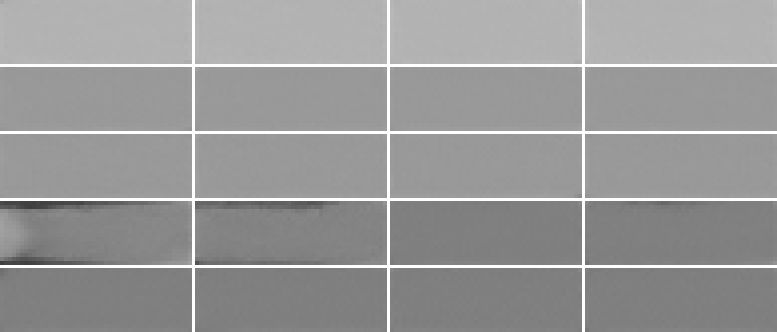
\includegraphics[width=\textwidth]{figures/ch10_v07_diffusion_candidates.png}
 \caption{По четыре volume-projected кандидата для каждого из пяти невидимых test conditions. Строки соответствуют условиям, столбцы --- различным diffusion samples.}
 \label{fig:practical-v07-candidates}
\end{figure}

\subsection{Разнообразие и степень бинарности}
\label{subsec:practical-v07-diversity}

Среднее попарное RMS-расстояние кандидатов внутри одного условия используется как простая проверка collapse. Его медиана по пяти условиям равна 0.0355. Следовательно, разные шумовые старты не сводятся к одному и тому же полю.

Для оценки серости используется
\begin{equation}
\label{eq:practical-v07-binarity}
 b(\rho)
 =
 \frac{1}{N_e}
 \sum_e
 4\rho_e(1-\rho_e).
\end{equation}
Здесь $b=0$ для бинарного поля и $b=1$ для однородного $\rho=1/2$. У generated candidates медиана $b$ равна 0.9599, а у терминальных test-топологий SIMP после такого же downsampling --- 0.2678. Это число не трактуется как критерий инженерной пригодности: оно только показывает, насколько diffusion output по серости похож на поздние SIMP-состояния.

Медианное RMS-расстояние сгенерированного кандидата до ближайшей терминальной train-топологии равно 0.3879. Эта величина также не доказывает новизну конструкции, но позволяет проверить, что sampling не сводится к точному воспроизведению одного сохранённого train-поля.

\subsection{Что V07 ещё не проверяет}
\label{subsec:practical-v07-boundary}

На этом шаге к generated candidates намеренно не применяется FEM. Поэтому из рисунка, разнообразия или noise MSE нельзя делать вывод о compliance, связности или механической допустимости. V07 заканчивается набором volume-feasible стартовых плотностей, а инженерная проверка переносится в V08:
\begin{equation}
\label{eq:practical-v07-next-pipeline}
 \begin{gathered}
  \text{conditional DDPM}
  \longrightarrow
  \text{volume projection}
  \\
  \longrightarrow
  \text{exact FEM}
  \\
  \longrightarrow
  \text{few-step SIMP refinement}.
 \end{gathered}
\end{equation}
Так генеративная модель отвечает только за предложение кандидатов, а физический смысл результата остаётся проверяемой частью вычислительного конвейера.

Локальный checkpoint и массив $80$ кандидатов не хранятся в Git. Их SHA256 вместе с параметрами обучения и sampling сохранены в 	exttt{v07\_diffusion\_results.json} и проверяются скриптом аудита.


\label{sec:practical-project-diffusion}

Третий проект меняет тип задачи. Теперь требуется по условию $c$ породить распределение разумных проектных кандидатов,
\begin{equation}
\label{eq:practical-conditional-generator}
 (z,c)
 \xmapsto{\ G_\phi\ }
 \rho_h^{\mathrm{gen}},
\end{equation}
где $z$ содержит случайность генерации. Условная диффузионная модель обучается на конструкциях, полученных из проверенного физического pipeline проекта~1. Сгенерированная плотность не объявляется решением до проверки точным FEM.

Практический контур проекта имеет вид
\begin{equation}
\label{eq:practical-generative-refinement}
 (z,c)
 \xmapsto{\ G_\phi\ }
 \rho_h^{\mathrm{gen}}
 \xmapsto{\ \mathrm{FEM}\ }
 J_h^{\mathrm{gen}}
 \longrightarrow
 \text{короткое SIMP-уточнение}
 \longrightarrow
 \rho_h^{\mathrm{ref}}
 \xmapsto{\ \mathrm{FEM}\ }
 J_h^{\mathrm{ref}}.
\end{equation}
Смысл такого эксперимента не в том, чтобы доказать превосходство генеративной модели над SIMP заранее. Проверяется более узкий практический вопрос: способен ли генератор быстро предлагать разнообразные начальные конструкции, которые после точной физической оценки и небольшого числа классических шагов дают конкурентный результат.

\subsection{Точная FEM-проверка всех кандидатов}
\label{subsec:practical-v08-screening}

V07 оставил $80$ допустимых по объёмной доле полей на сетке $48\times16$. Перед механической оценкой каждое поле поднимается на основную сетку без интерполяционного сглаживания:
\begin{equation}
\label{eq:practical-v08-upsample}
 \rho^{96\times32}_{2i+a,\,2j+b}
 =
 \rho^{48\times16}_{ij},
 \qquad
 a,b\in\{0,1\}.
\end{equation}
Средняя плотность при этом не меняется. После подъёма для каждого кандидата собирается точная матрица жёсткости с тем же $p=3$ и $E_{\min}/E_0=10^{-9}$, что и в проекте~1, и заново решается FEM-задача. Поэтому ranking строится не по изображению и не по нейросетевому surrogate, а по точному $J_h=F_h^{\trans}U_h$.

Для всех $80$ расчётов максимальная ошибка объёмной доли составила 1.00e-07, максимальная относительная FEM-невязка --- 2.40e-12. Пороговый путь материала от закрепления к нагруженной границе при $\rho\ge 0.5$ имели 6 из $80$ полей. Последнее число используется только как описательная проверка структуры: механическая допустимость всё равно определяется FEM.

\subsection{Одинаковый бюджет уточнения}
\label{subsec:practical-v08-budget}

В каждом test condition из $16$ полей выбираются четыре кандидата с наименьшим exact FEM compliance. Каждый из них получает ровно $30$ OC/SIMP updates с $r_{\min}=1.5$ и move limit $0.2$. Для контроля в том же условии выполняются те же $30$ updates от стандартной однородной инициализации $\rho=f_{\mathrm{vol}}$:
\begin{equation}
\label{eq:practical-v08-fixed-budget}
 \begin{aligned}
  \rho^{\mathrm{gen}}
  &\xrightarrow{\ 30\ \mathrm{OC}\ }
  \rho^{\mathrm{ref}},
  \\
  \rho^{\mathrm{uni}}
  &\xrightarrow{\ 30\ \mathrm{OC}\ }
  \rho_{30}^{\mathrm{uni}}.
 \end{aligned}
\end{equation}
Таким образом, сравнение warm start и обычного старта имеет одинаковый оптимизационный бюджет. Полностью сошедшееся terminal SIMP-состояние V04 используется отдельно как reference, а не как участник 30-шагового сравнения.

\subsection{Что получилось после 30 шагов}
\label{subsec:practical-v08-results}

\begin{table}[ht]
 \centering
 \small
 \begin{tabular}{c|r|r|r|r}
  $c$ & $J_{\mathrm{gen}}$ & $J_{\mathrm{ref}}$ & $J_{30}^{\mathrm{uni}}$ & $J_{\star}$\\
  \hline
  4 & 4342.92 & 339.59 & 340.28 & 335.70\\
  10 & 1517.15 & 246.12 & 247.39 & 240.09\\
  11 & 760.43 & 216.74 & 215.10 & 210.51\\
  19 & 465.90 & 192.35 & 192.11 & 189.18\\
  26 & 321.08 & 189.62 & 191.43 & 187.36\\
 \end{tabular}
 \caption{Для каждого невидимого условия: лучший сгенерированный кандидат до уточнения, лучший из четырёх после $30$ шагов, однородный $30$-шаговый контроль и сошедшийся SIMP reference из V04.}
 \label{tab:practical-v08-compliance}
\end{table}

В 3 из $5$ условий лучший diffusion warm start после одинаковых $30$ шагов имеет меньшую податливость, чем однородный $30$-шаговый контроль. Медиана отношения
\[
 \frac{J_{\mathrm{ref}}}{J_{30}^{\mathrm{uni}}}
 =
 0.9980,
\]
а медиана $J_{\mathrm{ref}}/J_{\star}$ равна 1.0168. Для самого однородного 30-шагового контроля медиана $J_{30}^{\mathrm{uni}}/J_{\star}$ равна 1.0217. Эти три числа разделяют эффект инициализации и эффект полного доведения SIMP до сходимости.

По всем $20$ уточняемым кандидатам медиана $J_{\mathrm{ref}}/J_{\mathrm{gen}}$ равна 0.1859. Следовательно, основное снижение compliance происходит уже внутри физического refinement, а роль DDPM проверяется более строго: даёт ли он старт, который при том же числе шагов оказывается лучше стандартного старта.

\begin{figure}[ht]
 \centering
 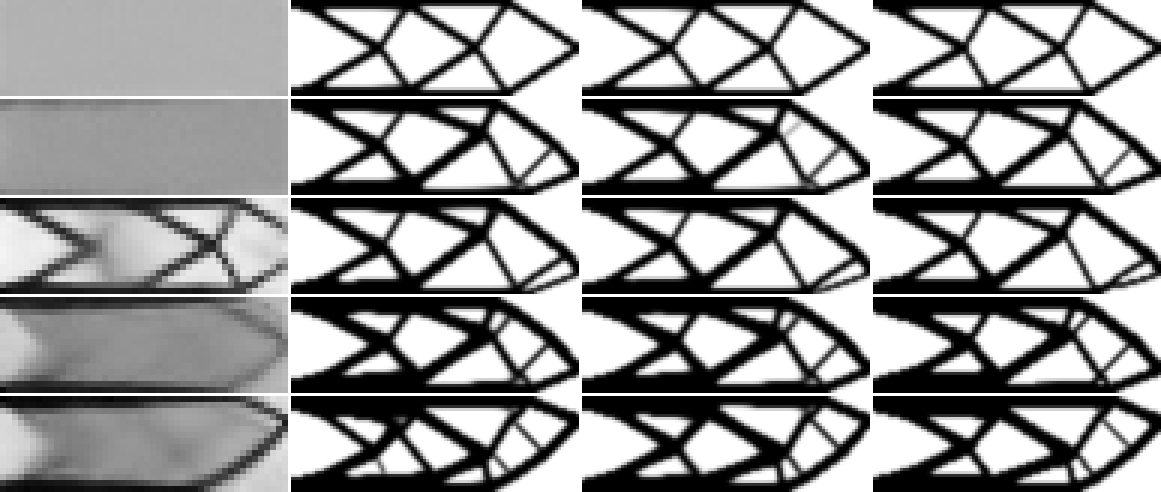
\includegraphics[width=\textwidth]{figures/ch10_v08_fem_refinement.png}
 \caption{Пять test conditions, по одному на строку. Столбцы слева направо: лучший кандидат после exact FEM screening, лучший diffusion warm start после $30$ SIMP-шагов, однородный $30$-шаговый контроль и terminal SIMP reference.}
 \label{fig:practical-v08-refinement}
\end{figure}

\subsection{Серость, связность и величина коррекции}
\label{subsec:practical-v08-structure}

Медианная бинарность выбранных diffusion starts равна 0.9222, после $30$ шагов --- 0.2174, а у terminal SIMP references --- 0.2046. Пороговая связность при $\rho\ge0.5$ наблюдалась у 2 из $20$ выбранных starts и у 20 из $20$ полей после refinement.

Медианное RMS-изменение плотности за $30$ шагов равно 0.4045. Это число важно вместе с compliance: если поле меняется существенно, нельзя приписывать конечную конструкцию одному генератору. В нашем pipeline DDPM предлагает начальное состояние, а SIMP и FEM отвечают за физическое исправление и окончательную оценку.

\subsection{Практический вывод проекта 3}
\label{subsec:practical-v08-conclusion}

На этом конечном test-наборе diffusion warm start даёт измеримое преимущество при одинаковом 30-шаговом бюджете. Это не утверждение о глобальном превосходстве DDPM, а результат ровно для пяти заранее отделённых условий.

При этом fixed-budget результат нельзя смешивать с fully converged reference. Даже лучший diffusion warm start после 30 шагов в медиане остаётся выше сошедшегося V04 reference, поэтому короткое уточнение не заменяет полную оптимизацию.

Итоговый вычислительный контракт проекта~3 теперь полностью проверяем:
\begin{equation}
\label{eq:practical-v08-final-pipeline}
 \begin{gathered}
  c
  \longrightarrow
  \text{conditional DDPM candidates}
  \longrightarrow
  \text{exact FEM ranking}
  \\
  \longrightarrow
  \text{fixed-budget SIMP refinement}
  \longrightarrow
  \text{final exact FEM}.
 \end{gathered}
\end{equation}
Генератор не получает права объявлять конструкцию хорошей самостоятельно; это право остаётся у физического расчёта и явно заданного критерия сравнения.

\section{Сквозное сравнение и границы применимости}
\label{sec:practical-cross-project-comparison}

После трёх проектов сравниваются три режима вычисления одной и той же инженерной задачи. Первый режим решает физику и оптимизацию напрямую; второй заменяет многократный физический расчёт обучаемым оператором там, где его ошибка допустима; третий использует обучаемую модель для поиска кандидатов, но возвращает точную физику в окончательную проверку. Сравнение проводится по качеству конструкции, численной допустимости, времени и области условий, на которой метод был проверен.

Главный результат главы --- воспроизводимый вычислительный маршрут. Для нового условия задачи должно быть явно указано, как формируется $c$ и какой решатель вычисляет $U_h$. Обучаемое приближение отделяется от точного расчёта, а окончательное качество всегда определяется заранее выбранным физическим критерием.

\subsection{Три разных роли в одном вычислительном контуре}
\label{subsec:practical-v09-three-roles}

Три проекта нельзя сравнивать как три взаимозаменяемых решателя. В первом проекте FEM вычисляет физический ответ, а SIMP непосредственно меняет конструкцию. Во втором проекте FNO приближает отображение $\rho_h,c\mapsto U_h$ и потому может ускорять повторную оценку поля, но не получает права заменить уравнение равновесия. В третьем проекте DDPM вообще не решает механику: он предлагает стартовые плотности, после чего точный FEM и SIMP возвращаются в контур.

Для основной консоли классический SIMP уменьшил податливость с 1848.075 до 233.550, то есть на 87.36\%. Сходимость потребовала 77 итераций. Этот результат остаётся baseline, потому что каждая оптимизационная итерация опирается на тот же проверенный FEM, которым затем оцениваются ML-кандидаты.

\subsection{Что действительно дал нейронный оператор}
\label{subsec:practical-v09-fno-role}

На condition-level test медианная относительная ошибка поля FNO равна 3.68\%, а медианная ошибка податливости --- 7.33\%. Один CPU-forward оказался примерно в 5.27 раза быстрее полного FEM-расчёта на сетке $96\times32$. Для screening важнее, что внутри test-условий FNO сохранил правильный порядок по податливости в 94.7\% пар и выбрал лучший snapshot в 4 случаях из 5.

Однако медианная невязка равновесия равна 6.45e+01, а zero-shot ошибка поля на $192\times64$ --- 35.95\%. Поэтому практический вывод узкий: FNO полезен для быстрого предварительного ранжирования на проверенном распределении условий и разрешении, но окончательная инженерная метрика должна возвращаться к exact FEM.

\subsection{Что действительно дала условная диффузия}
\label{subsec:practical-v09-ddpm-role}

DDPM генерирует разнообразные поля, но raw candidates не являются готовыми конструкциями. До refinement при пороге $\rho=0.5$ связны только 6 из 80 полей. После exact FEM screening и $30$ SIMP-шагов для top-$4$ кандидатов связны уже 20 из 20. Медианная бинарность меняется с 0.960 до 0.217, тогда как у fully converged terminal reference она равна 0.205.

Главная проверка warm start сравнивает одинаковый бюджет в $30$ SIMP-шагов. Diffusion initialization лучше обычной однородной инициализации в 3 из 5 условий, но медианное отношение
\begin{equation}
\label{eq:practical-v09-warmstart-ratio}
 \frac{J_{\mathrm{diffusion}+30}}
 {J_{\mathrm{uniform}+30}}
 =
 0.99798.
\end{equation}
Это преимущество невелико. Одновременно
\begin{equation}
\label{eq:practical-v09-terminal-gap}
 \frac{J_{\mathrm{diffusion}+30}}
 {J_{\mathrm{terminal}}}
 =
 1.01677,
\end{equation}
а медианное RMS-изменение плотности за refinement равно 0.404. Следовательно, генератор влияет на начальную точку, но основную перестройку до механически пригодной конструкции по-прежнему выполняет SIMP.

\subsection{Сквозной практический маршрут}
\label{subsec:practical-v09-route}

Полученный вычислительный маршрут можно записать без смешения ролей:
\begin{equation}
\label{eq:practical-v09-final-route}
 \begin{gathered}
  c,\rho
  \longrightarrow
  \text{FNO screening}
  \longrightarrow
  \text{короткий список},
  \\
  c
  \longrightarrow
  \text{DDPM candidates}
  \longrightarrow
  \text{FEM screening}
  \longrightarrow
  \text{SIMP refinement},
  \\
  \text{любой финальный кандидат}
  \longrightarrow
  \text{exact FEM}.
 \end{gathered}
\end{equation}
Первый ML-блок ускоряет оценку, второй расширяет поиск начальных конструкций, но физическая проверка в обоих случаях возвращается в точный решатель. Именно это является общим инженерным выводом трёх проектов.

\subsection{Стоимость и границы утверждений}
\label{subsec:practical-v09-cost-scope}

Обучение FNO заняло 24.48 мин CPU-времени, обучение DDPM --- 9.55 мин, а полный V08 screening и refinement --- 1.92 мин. Эти времена относятся к одному ноутбуку и не являются оценками асимптотической сложности. Они нужны только для воспроизводимого сравнения внутри данного эксперимента.

Полученные числа не дают оснований утверждать инвариантность FNO к разрешению, универсальное преимущество диффузионной инициализации или причинное влияние отдельных параметров нагрузки. В тестовой части всего пять новых условий, а перенос FNO на более тонкую сетку заметно ухудшил точность. Поэтому результат главы скромнее и практически важнее: обучаемые модели можно включать в расчётный контур только с возвратом к точной физической проверке.

\subsection{Воспроизводимость V09}
\label{subsec:practical-v09-reproducibility}

Численные выводы V03--V08 собраны в сводном файле V09. Отдельный манифест хранит контрольные суммы пяти файлов результатов и пяти локальных артефактов: датасета, двух контрольных точек моделей и двух массивов кандидатов. Новых экспериментов V09 не добавляет. На этапе CLOSE остаются только итоговый аудит, сборка PDF и создание единственного архива.
